\documentclass[5pt]{article}
\usepackage{multicol,multirow}
\usepackage{graphicx} % Required for inserting images
\usepackage[margin=0.75cm]{geometry}
\usepackage{xcolor}
\usepackage{amsmath}
\usepackage{mathtools}
\usepackage{empheq}
\usepackage{amsfonts}
\usepackage{minted}
\usepackage{tkz-berge}
\usepackage{graphicx}
\graphicspath{ {./fig_1/} }

\usepackage{tikz}
\usetikzlibrary{calc,patterns,angles,quotes}


\definecolor{LightGray}{gray}{0.9}

\DeclarePairedDelimiter\abs{\lvert}{\rvert}%
\DeclarePairedDelimiter\norm{\lVert}{\rVert}%

\makeatletter
\let\oldabs\abs
\def\abs{\@ifstar{\oldabs}{\oldabs*}}

\makeatletter
\newcommand*{\rom}[1]{\expandafter\@slowromancap\romannumeral #1@}
\makeatother

\begin{document}
\begin{center}
     \Large{\textbf{General Physics 1}}\\
     \small{Class: Phys 1110}\hfill\small{\textcopyright Maximilien Notz \the\year{}}
     \noindent\rule{20.2cm}{0.4pt}
\end{center}

\begin{multicols}{3}
\setcounter{secnumdepth}{0}

\section{Definitions}
\begin{tabular}{ll}
Speed & $v =\abs{\frac{dx}{dt}}$\\[6pt]
Velocity & $\vec{v} = \frac{d\vec{s}}{dt}$\\[6pt]
Acceleration & $\vec{a} = \frac{d\vec{v}}{dt}$\\[6pt]
Force & $\vec{F} = m\vec{a}$
\end{tabular}

\section{Vectors}
\begin{tabular}{ll}

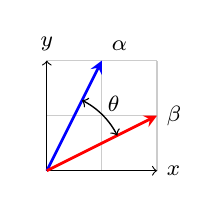
\begin{tikzpicture}[scale=0.70]
  \draw[thin,gray!40] (0,0) grid (2,2);
  \draw[->] (0,0)--(2,0) node[right]{\footnotesize$x$};
  \draw[->] (0,0)--(0,2) node[above]{\footnotesize$y$};
  \draw[line width=1pt,blue,-stealth](0,0)--(1,2) node[anchor=south west]{};
  \draw[line width=1pt,red,-stealth](0,0)--(2,1) node[anchor=south]{}; 
  \draw [line width=0.5pt]
    (2,1) coordinate (a) node[right] {\footnotesize$\beta$}
    (0,0) coordinate (b) node[left] {}
    (1,2) coordinate (c) node[above right] {\footnotesize$\alpha$}
    pic["\footnotesize$\theta$", draw=black, <->, angle eccentricity=1.2, angle radius=1cm]
    {angle=a--b--c};
\end{tikzpicture} & 
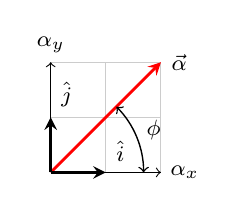
\begin{tikzpicture}[scale=0.70]
  \draw[thin,gray!40] (0,0) grid (2,2);
  \draw[->] (0,0)--(2,0) node[right]{\footnotesize$\alpha_x$};
  \draw[-stealth, line width=1pt,red] (0,0)--(2,2) node[right, black]{\footnotesize$\vec\alpha$};
  \draw[->] (0,0)--(0,2) node[above]{\footnotesize$\alpha_y$};
  \draw[line width=1pt,black,-stealth](0,0)--(1,0) node[anchor=south west]{\footnotesize$\hat{i}$};
  \draw[line width=1pt,black,-stealth](0,0)--(0,1) node[anchor=south west]{\footnotesize$\hat{j}$};
    \draw [ line width=0.5pt]
    (2,0) coordinate (a) node[] {}
    (0,0) coordinate (b) node[] {}
    (2,2) coordinate (c) node[] {}
    pic["\footnotesize$\phi$", draw=black, <->, angle eccentricity=1.2, angle radius=1.18cm]
    {angle=a--b--c};
\end{tikzpicture}\\
Norm 2 & $||\vec{\alpha}||_2 = \sqrt{\alpha_1^2+\dots+\alpha_n^2}$\\
addition & $\vec{\alpha}+\vec{\beta}=\big(\begin{smallmatrix}
  \alpha_x + \beta_x  \\
  \alpha_y+ \beta_y
\end{smallmatrix}\big)$ \\[6pt]
Dot Product & $\vec{\alpha}\cdot\vec{\beta}=||\vec{\alpha}||\: ||\vec{\beta}||\cos{\theta}$\\
  & $=\alpha_x\beta_x+\alpha_y\beta_y$\\
Cross Product & $||\vec{\alpha}\times\vec{\beta}||=||\alpha||\;||\beta||\sin{\theta}$\\
Unit Vector & $\vec{\alpha}=x\hat{i}+ y\hat{j}$\\
X component & $\alpha_x = \vec{\alpha}\cdot\hat{i}=||\vec{\alpha}||\cos{\phi}$\\
Y component & $\alpha_y = \vec{\alpha}\cdot\hat{j}=||\vec{\alpha}||\sin{\phi}$\\
\end{tabular}


\section{Newton laws}
\subsection{N \rom{1}}
$\sum{\vec{F} = \vec{F_{net}}}$
\subsection{N \rom{2}}
$\vec{F}=m\vec{a}$
\subsection{N \rom{3}}
let $\vec{F_{ab}}$ be the force \textbf{on a from b} and $\vec{F_{ba}}$ be the force \textbf{on b from a}.\\
$\vec{F_{ab}}=\vec{-F_{ba}}$


\section{Kinematics}
$v_1=v_0+at$\\
$v_1^2=v_0^2+2a\Delta x$\\
$x_1=x_0 + vt + \frac{1}{2}at^2$

\section{Circular Motion}
\begin{tabular}{ll}
Period($T$) & time for 1 revolution.\\
Circle radius & r\\
Speed & $||\Vec{v}||=\dfrac{2\pi r}{T}$
\end{tabular}

\section{Work(W) \& Energy(E)}
\begin{tabular}{ll}
Work & $W_{1\to 2}=\int_{x_1}^{x_2}\Vec{F}_{Net}\cdot d\Vec{x}$\\
W-K Thm & $W_{Net}=\Delta K$\\
Kinetic E & $K=\frac{1}{2}m\Delta v^2$\\
Potential E & $\Delta U_{Gravity}=mg\Delta h$\\
Mechanical E & $E_{Mechanical}=K+U$\\
\footnotesize{Conservative $E_{mec}$} & $\Delta K+\Delta U=0$\\
& $\Delta E_{Mec}=\sum W_{NC}$\\
& $\Delta U = - W_{A\to B}$\\
& $F(x)=-\frac{du}{dx}$
\end{tabular}
Conservative forces  are gravity and springs.

\subsubsection{Gravity}
\begin{tabular}{ll}
$G$ & The gravitational constant\\
$M_E$ & The mass of the Planet\\
$m$ & The mass of the body\\
$r_1$ & the initial distance between the body\\ &and the planet.\\
$r_2$ & the final distance between the body\\ &and the planet.\\
\end{tabular}
\\
\begin{tabular}{ll}
Force & $F_{Grav}=G\dfrac{m_1m_2}{r^2}$\\
Work  & $W_{1\to 2}=GM_Em\left(\frac{1}{r_2}-\frac{1}{r_1}\right)$\\
Close to Earth & $W=-gm\Delta y$\\
potencial energy & $U=-\dfrac{GMm}{r}$\\
Escape speed & $v_{esc}=\sqrt{\dfrac{2GM}{R}}$
\end{tabular}

\subsubsection{Kepler Laws}
\subsection{K \rom{1}}
A planet's orbit is an ellipse with the sun at one focus.

\subsection{K \rom{2}}
\includegraphics[scale=0.5]{fig_1}

\subsection{K \rom{3}}
For a planet around the sun, the period T and the mean distance r from the sun are related by $\frac{T^2_A}{r^3_A} = \frac{T^2_B}{r^3_B}$. This means that planets further from the sun (larger r)have longer orbit (longer T).

\section{Momentum}
\begin{tabular}{ll}
Momentum Def 1  & $\vec{p}=m\vec{v}$\\
Momentum Def 2  & $\Vec{F}=\frac{d\vec{p}}{dt}$\\
center of mass & $\vec{R}_{CM}=\dfrac{\sum^N_{i=l}m_i\vec{r}_i}{M_{total}}$\\
Total Momentum & $\Vec{P}_{total}=M_{total}V_{CM}$\\
\end{tabular}

\section{Rotational Kinematic}
\begin{tabular}{ll}
Arc Length\footnotesize{(R=radius)} & $s=R\theta$\\
(\footnotesize{in degrees}) & $s=2\pi R \frac{\theta}{360}$\\
Angular Velocity  & $\omega=\frac{d\theta}{dt}$\\
Angular Acceleration  & $\alpha=\frac{d\omega}{dt}$\\
Tangential(Tan.) speed & $v_{tan}=R\omega$\\
Tan. Acceleration & $a_{tan}=R\alpha$\\
Moment Of Inertia & $I=\sum{m_ir_i^2}$\\
 & $I=\int{r^2\; dm}$\\
Rot. Kinetic Energy & $K_{system}=\frac{1}{2}I\omega^2$\\
Torque ($\tau$) & $|\tau|=r\cdot F_\perp$\\
 & $|\tau|=rF\sin{\theta}$\\ 
 & $\vec{\tau}=\Vec{r}\times\Vec{F}$\\ 
& $\tau_{net}=\sum\tau$\\
\footnotesize{($F=ma$ rot. equivalent)} & $\tau=I\:\alpha$\\
Angular momentum & $\vec{L}=\vec{r}\times\Vec{p}$\\
\footnotesize{ If $\tau_{ext}=0$ then} & $L_{tot}=I\omega$\\
\end{tabular}


\section{Static Equilibrium}
$\sum F_x=0$, $\sum F_y=0$, $\sum\tau=0$


\section{Simple Harmonic Motion}
\begin{tabular}{ll}
Pendulum & $x(t)=x_0\cos{\omega t}$\\
Mass-spring & $\omega=\sqrt{\frac{k}{m}}$\\
 & $T=2\pi\sqrt{\frac{m}{k}}$\\
\end{tabular}


\section{Wave Speed}
Transversal W. Ex: Water.\\
Longitudinal W. Ex: Sound.\\
\begin{tabular}{ll}
Period & $T=f^{-1}$\\
Speed & $v=\frac{\lambda}{T}=\lambda f$\\
Displacement & $y(x, t=0)=A\sin(2\pi\frac{x}{\lambda})$\\
 & $=Asin(kx)$\\
& $y(x,t)=A\sin(2\pi(\frac{x}{\lambda}+\frac{t}{T}))$\\
Ang. Freq. & $\omega=\frac{2\pi}{T}$\\
Interference & $y_{tot}(x,t)=y_1(x,t)+y_2(x,t)$\\
\end{tabular}

\subsection{Standing Waves}
\begin{tabular}{ll}
Integer & $n$\\
Total length & $L=n\frac{\lambda}{2}$\\
\end{tabular}

\subsection{Fluid}
\begin{tabular}{ll}
Area & A\\
Volume & V\\
Density & $\rho=\frac{m}{V}$\\
Pressure & $p=\frac{F_{\perp}}{A}$\\
& $\Delta p=\rho g\Delta h$\\
Archimedes P.& $F_{buoy}=m_{fluid}g=\rho Vg$\\
\end{tabular}

\section{Constants}
$c_{light}=299\:792\:458\;ms^{-1}$\\
$c_{sound}=343\;ms^{-1}$\\
$g=9.807\;\; ms^{-2}$\\
$G=6.6743\cdot 10^{-11}\;\; m^3 kg^{-1} s^{-2}$

\section{Other}
\begin{tabular}{ll}
Change  & $\Delta v^2=(v_f^2-v_i^2)$\\
Spring Force & $\vec F = -k\vec x$\\
Spring work & $W_{1\to 2}=-\frac{1}{2}k(x_2^2-x_1^2)$

\end{tabular}


\end{multicols}
\end{document}